\documentclass{article}
\usepackage[utf8]{inputenc}
\usepackage{enumitem}
\usepackage{fancyhdr}
\usepackage{titling}
\usepackage[]{mcode}
\usepackage{amsmath}
\usepackage{hyperref} %for hyper links
\usepackage[T1]{fontenc}
\usepackage{titling}
\usepackage{graphicx} %package to manage images
\usepackage{caption} % subfigure package
\usepackage{subcaption} % subfigure package
\usepackage{array} %for table formatting

%page size
\usepackage{geometry}
\geometry{
	a4paper,
	total={170mm,257mm},
	right=30mm,
	left=30mm,
	top=25mm,
}

\graphicspath{ {/images} } %path to images folder

\setlength{\droptitle}{-10em}   % This is your set screw

\newcommand{\vect}[1]{\boldsymbol{#1}} % to make vectors

%front page
\setlength{\droptitle}{2em}   % This is your set screw

\def\subject{MACHINE LEARNING AND PATTERN RECOGNITION}
\def\matricno{s1569105}
\def\exmno{B076165}

\title{\subject\\Assignment 1}
\date{November 2015}
\author{Matriculation number - \matricno\\Examination number - \exmno}

\begin{document}

\maketitle
	\section{The Next Pixel Prediction Task}
		\section*{Note} 
			 For all code snippets in the part 1 it is assumed that I have loaded imgregdata.mat file via matlab terminal before I ran the scripts. For the tasks starting from 1.3 it is also assumed that I have loaded NetLab and welltrainedMLP.mat file.\\ I don't calculate RMSE upper and lower bounds for cross-validation because it is quite difficult to achieve this with default matlab crossval function. But in such cases I report RMSE with bounds on the test set.
		\subsection{Data preprocessing and visualization}
			 \begin{enumerate}[label=(\alph*)]
			 	\item
				 	\begin{figure}[htp]
				 		\centering
				 		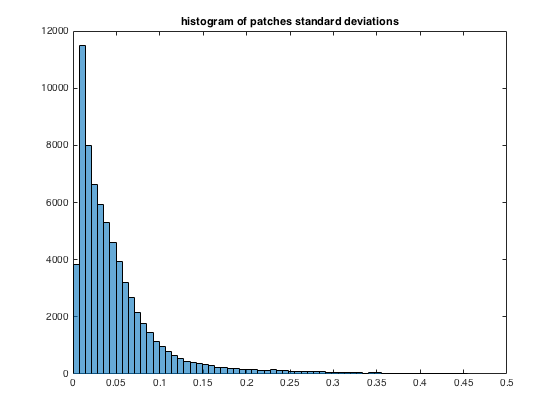
\includegraphics[width=12cm]{images/p1-1-a_std_hist}
				 		\caption{histogram of standard deviations in the xtr dataset after normalisation}
				 		\label{fig:p1-1-a_std_hist}
				 	\end{figure}
				 	From the figure \ref{fig:p1-1-a_std_hist} we can see that after the peak on the second bin (associate it with deviation around 1 discrete pixel value) the number of patches declines exponentially as  standard deviation increases . We can conclude that most of patches have standard deviation between 0 and 0.05. It can be confirmed from subtask c. 52739 patches which is more than 75\% of our initial dataset have standard deviation within 0 and 0.0635 range, and 0.0635 is quite small standard deviation. Therefore, most of the patches are flat ones. \\
				 	The distribution can be described by that family of distribution $P(t) \propto t^{\alpha} exp(-\beta t)$, 
				 	The maximum possible value of standard deviation is $\frac{max. - min.}{2}$, so in our case after normalisation it is $\frac{1 - 0}{2}= 0.5$. Our threshold to distinguish discrete values of pixels is $\frac{1}{64} = \approx 0.0156$ so that values between 0 and 0.0156 will be regarded as discrete intensity of zero and between 63 * 0.0156 and 1 will be discrete intensity of 63. Because most of the patches are flat one we can approximately describe each such patch as Gaussian. That is why we can say that approximately 95\% of pixels will be within two standard deviations from mean of the patch. Due to the fact that each bin corresponds to the standard deviation by the equation $bin-standard-deviation = bin-index * bin-width$ and, therefore, two standard deviations $2 * bin-standard-deviation = bin-index * 2 * bin-width$. So by choosing bin-width as half of our threshold 0.0156 we can associate each bin with discrete (original pixel value) value of 2 standard deviations. That is why it will be possible to say that for the patch in the first bin most of the pixels are different from the mean value only by 1 discrete value of intensity, for second bin it will be 2 discrete value of intensity, etc until we reach non-flat patches. And $bin-width = threshold * 0.5 = 0.5/64$ so we should choose 64 as number of our bins.
				 	Code snippet to plot histogram:
				 	\lstinputlisting{code/tsk1_1_a.m}
				 	
				\item
					I would choose the mean of all pixels in the patch as simple predictor for flat patches. Given the definition of flat patches the intensity of the i'th pixel in the flat patch should be something like this $f_{i}(\vect{x_{all\ other\ pixels}}) = const_{this flat\ patch} + o(\vect{x_{all\ other\ pixels}})$ where $o(\vect{x_{all\ other\ pixels}})$ is small function in comparison to $const_{flat\ patch}$, and $o(\vect{x_{all\ other\ pixels}})$  mean and standard deviation over all pixels in the patch are 0 and $\sigma_{flat\ patch}$ respectively. For flat patches the following is true $\sigma_{flat \, patch} \leq \sigma_{flat \, pach \, max}$. So it is natural to propose  $const_{this flat\ patch}$ as our prediction, which can be received by calculating mean over all pixels in the flat patch\\
					The performance of this simple predictor can be estimated by considering extreme case when after normalisation (all pixel values between 0 and 1) most pixels are zeroes and small portion of pixels are ones (correspond to original intensity of 63). Let $N-m$ be number of zeros and let $m$ be number of ones and I denote $\mu$ as mean. 
					\begin{gather*}
						m < N - m
						\\
						\mu = \frac{(N - m) * 0 + m * 1}{N} = \frac{m}{N}
						\\
						\sigma^2 =\frac{1}{N}[(N - m) (0 - \frac{m}{N})^2 + m(1 - \frac{m}{N})^2]
						\\
						= \frac{(N - m)m^2}{N^3} + \frac{m(N - m)^2}{N ^ 3}
						\\
						N^3\sigma^2 = m^2N - m^3 + mN^2 - 2m^2N + m^3 
						\\
						= mN^2-m^2N
						\\
						m^2 - mN + N^2\sigma^2 = 0
						\\
						m = \frac{N}{2}(1 - \sqrt{1 - 4 \sigma ^ 2})\quad\text{(minus because our case is $m < N - m$ )}
					\end{gather*}
					putting $\sigma_{flat \, pach \, max} = \frac{4}{63} \approx 0.0635$ instead of $\sigma$ and using $N = 1032$ we get
					\begin{gather*}
						m = \frac{1032}{2}(1 - \sqrt{1 - 4 * 0.0635^2}) \approx 4.178
					\end{gather*}
					rounding m to the closest integer we receive $m = 4$. \\Thus, in most extreme case of flat patch we can have 4 ones (correspond to original pixel intensity of 63) and 1028 zeros, so it is natural that we want to predict zero as discrete value of our target pixel.  The mean gives us $\mu = \frac{1028 * 0 + 1 * 4} {1032} \approx 0.0038$. Dividing range between 0 and 1 by 64 we get 0.0156 as our threshold to distinguish discrete pixel values. 0.0038 lies between 0 and 0.0156 so our mean value would correspond to 0 as the discrete value of our target pixel and that is what we wanted.
				\newpage
				\item
				 	\begin{figure}[t]
				 		\centering
				 		\caption{patch images}
				 		\label{fig:patch_images}
						\begin{subfigure}{0.5\textwidth}
											      	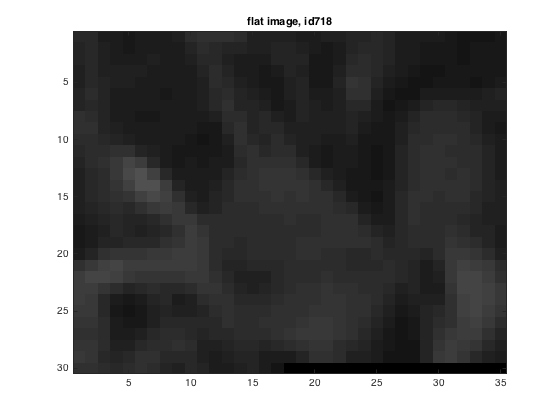
\includegraphics[width=\linewidth]{images/p1-1-c_flat}
											      	\caption{flat patch image}
											      	\label{fig:flat_patch_image}
						\end{subfigure}%
						\begin{subfigure}{0.5\textwidth}
											      	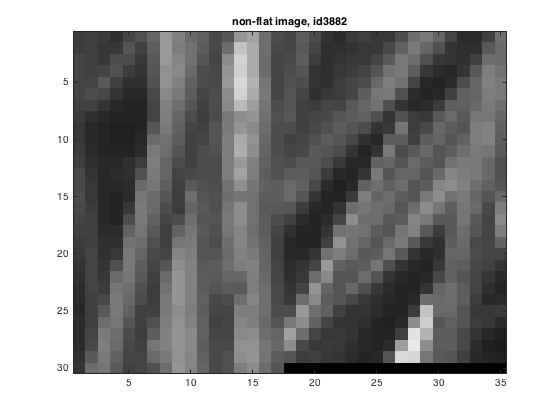
\includegraphics[width=\linewidth]{images/p1-1-c_non_flat}
											      	\caption{non-flat patch image}
											      	\label{fig:non-flat_patch_image}
						\end{subfigure}%
				 	\end{figure}
					 Code snippet to show patch images on figure \ref{fig:patch_images}:
				 	 \lstinputlisting{code/tsk1_1_c.m} 
			\end{enumerate}		
		\subsection{Linear regression with adjacent pixels}
			\begin{enumerate}[label=(\alph*)]
				\item
				 	\begin{figure}[t]
				 		\caption{}
				 		\begin{subfigure}{0.5\textwidth}
				 			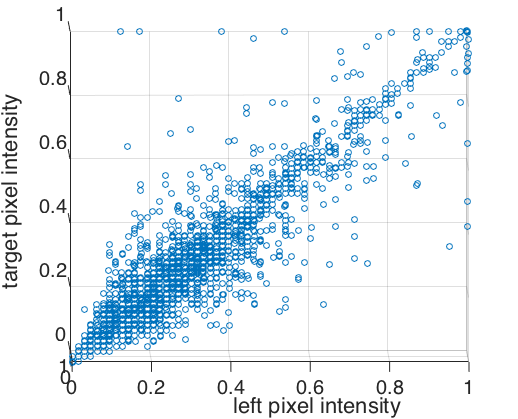
\includegraphics[width=\linewidth]{images/p1-2-a_left_target.png}
				 			\caption{5000 data points from xtr\_nf and ytr\_nf}
				 			\label{fig:p1-2-a_left_target}
				 		\end{subfigure}
				 		\begin{subfigure}{0.5\textwidth}
				 			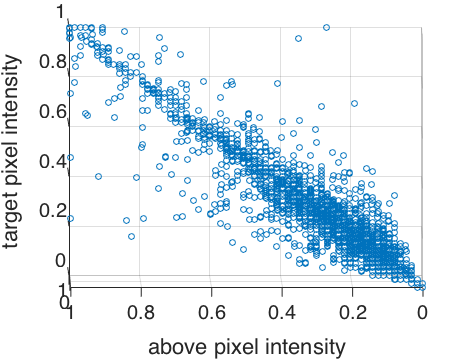
\includegraphics[width=\linewidth]{images/p1-2-a_above_target.png}
				 			\caption{5000 data points from xtr\_nf and ytr\_nf}
				 			\label{fig:p1-2-a_above_target}
				 		\end{subfigure}		
				 		\begin{subfigure}{0.5\textwidth}
				 			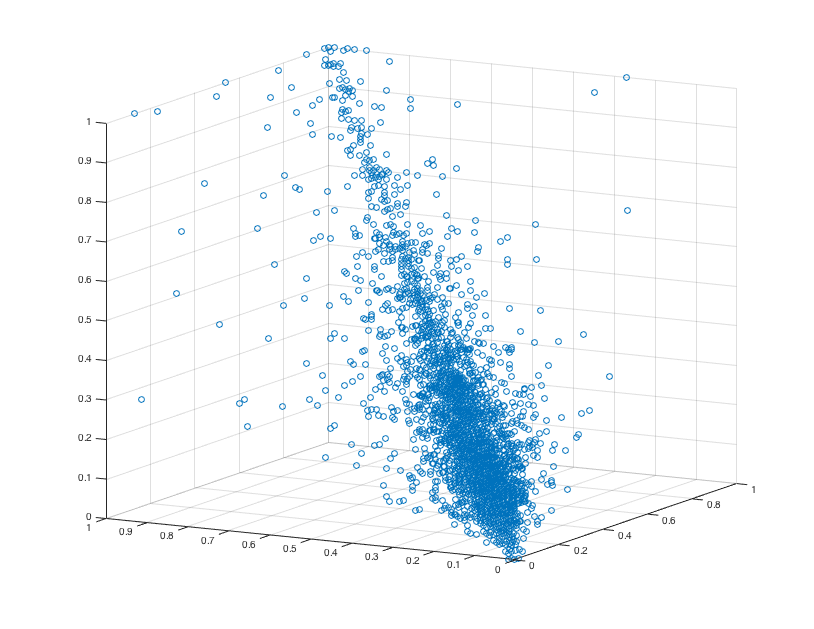
\includegraphics[width=\linewidth]{images/p1-2-a_closest_pixels.png}
				 			\caption{5000 data points from xtr\_nf and ytr\_nf}
				 			\label{fig:p1-2-a_closest_pixels}
				 		\end{subfigure} 
				 		\begin{subfigure}{0.5\textwidth}
				 			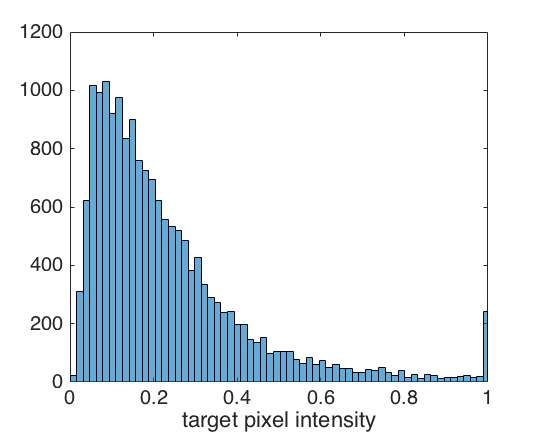
\includegraphics[width=\linewidth]{images/p1-2-a_target_hist.png}
				 			\caption{histogram of target pixel intensity on the full training set}
				 			\label{fig:p1-2-a_target_hist}
				 		\end{subfigure} 		
				 	\end{figure}	
					I used 5000 training points from xtr\_nf and ytr\_nf to figure \ref{fig:p1-2-a_closest_pixels}. From it we can see that x(j, end), x(j, end - 34), y(j) are strongly positively correlated. However, there is some  number of deviations from this trend. It seems that these deviations are normally distributed because the bigger distance from general trend the fewer instances we have on the plot. By looking at the figures \ref{fig:p1-2-a_left_target}, \ref{fig:p1-2-a_left_target} and the huge bulb like distribution in the beginning of the figure  \ref{fig:p1-2-a_closest_pixels}  it may seem that $\sigma_{\eta}$ standard deviation of the noise $\eta$ in this expression for linear regression model $y = \vect{w}^{T}\vect{x} + \eta \quad \eta \approx Gaussian(0, \sigma_{\eta})$ in reality is not a constant and it depends heavily on the target pixel value. But it happens due to the fact that it is much more likely to have darker target pixels, and therefore we have more samples from our distribution in the darker area. This can be seen on the histogram \ref{fig:p1-2-a_target_hist}, and I have slightly inclined figures  \ref{fig:p1-2-a_left_target}, \ref{fig:p1-2-a_left_target} so it is easier to see the number of data points.\\
					Code snippet for scatter plot:
					\lstinputlisting{code/tsk1_2_a.m} 
				\item
					Derivation of this solution can be taken from MLPR lecture 7 slides 8-11 \href{http://www.inf.ed.ac.uk/teaching/courses/mlpr/2015/slides/07_regression.pdf}{link}. The solution for weights from there is:
					\begin{gather*}
					\hat{\vect{w}} = (\Phi^T \Phi)^{-1} \Phi^T \vect{y}
					\end{gather*}
					In our notation matrix $\Phi$ will become:
					\begin{gather*}
						\Phi = X = 
						\begin{pmatrix}
						1, x(1, end), x(1, end - 34)\\
						1, x(2, end), x(2, end - 34)\\
						\ldots \\
						1, x(N, end), x(N, end -34)
						\end{pmatrix} \\
						\hat{\vect{w}} = (X^T X)^{-1} X^T \vect{y}
					\end{gather*}
					where N is a number of training data points and x is our dataset (it will be xtr\_nf in the next task)\\
					I asked professor Chris Williams and he said there is no need to repeat all derivations from MLPR lecture (what new can we add there anyway?).
				\item
					After training the weights are:
					\begin{center}
						\begin{tabular}{| c | c | c |}
							\hline
							bias & left pixel & above pixel \\ \hline
							0.0026  & 0.4606 & 0.5241 \\ 
							\hline
						\end{tabular}
					\end{center}					
					the RMSE for test and training sets:
					\begin{center}
						\begin{tabular}{| c | c | c |}
							\hline
							\, & Training set & Test set \\ \hline
							RMSE  & $0.0506 \pm 0.0010$ & $0.0503 \pm 0.0017$ \\ 
							\hline
						\end{tabular}
					\end{center}
				 	\begin{figure}[t]
				 		\centering
				 		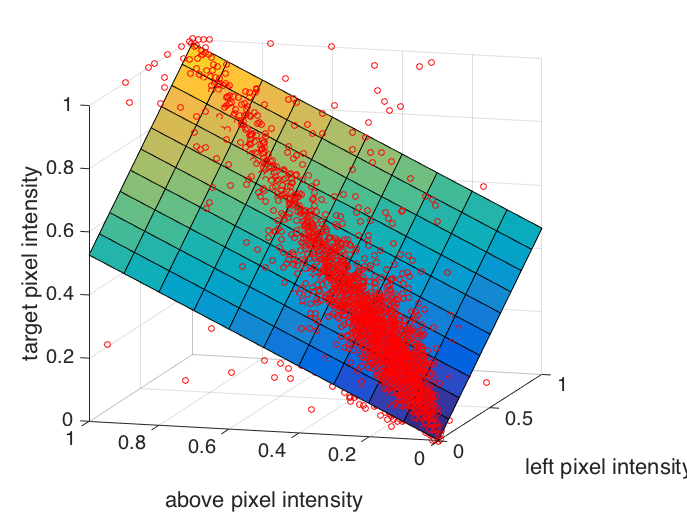
\includegraphics[width=10cm]{images/p1-2-c}
				 		\caption{plot of the linear regression function after training along with test data points}
				 		\label{fig:p1-2-c}
				 	\end{figure}
					Taking bounds into consideration we can see that the performance on training and test is almost the same. That is why we can conclude that linear regression is not over-fitting the data in this problem. It can be seen from figure \ref{fig:p1-2-c} that indeed there is strong positive correlation between adjacent pixels and target value pixel. \\
					Code snippet to get linear regression predictor (will also be used afterwards):
					\lstinputlisting{code/cs_linear_regression.m} 
					Code snippet to compute root mean square error (RMSE) with bounds (implementation pointed out by professor Chris Williams), which correspond to standard errors of mean square error(MSE)  (will also be used  afterwards):
					\lstinputlisting{code/cs_rmse.m}
					Code snippet to show rmse on training and test set with bounds (will also be used  afterwards):
					\lstinputlisting{code/show_rmse.m}
					Code snippet for this task:
					\lstinputlisting{code/tsk1_2_c.m}
			\end{enumerate}
		\subsection{RBF regression with adjacent pixels}
			\begin{enumerate}[label=(\alph*)]
				\item
				 	\begin{figure}[t]
				 		\caption{Root Mean Square Error against number of radial basis functions used}
				 		\begin{subfigure}{0.5\textwidth}
				 			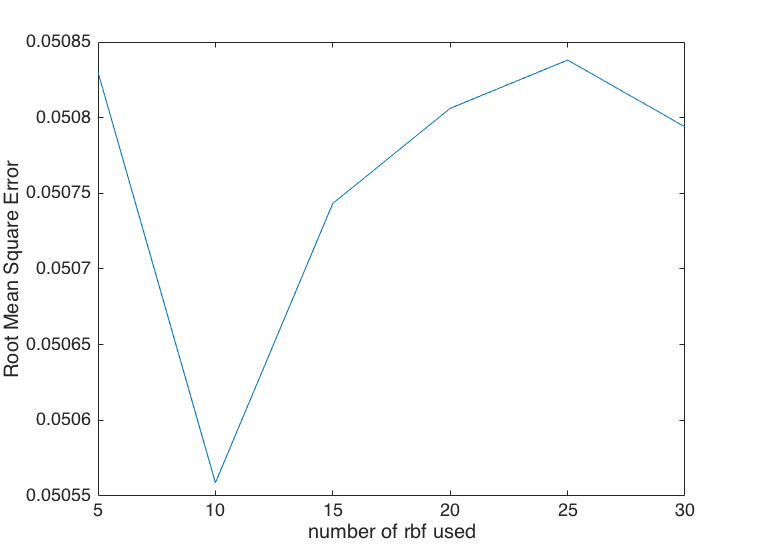
\includegraphics[width=\linewidth]{images/p1-3-a_5_30.png}
				 			\caption{}
				 			\label{fig:p-1-3-a_a}
			 			\end{subfigure}
				 		\begin{subfigure}{0.5\textwidth}
				 			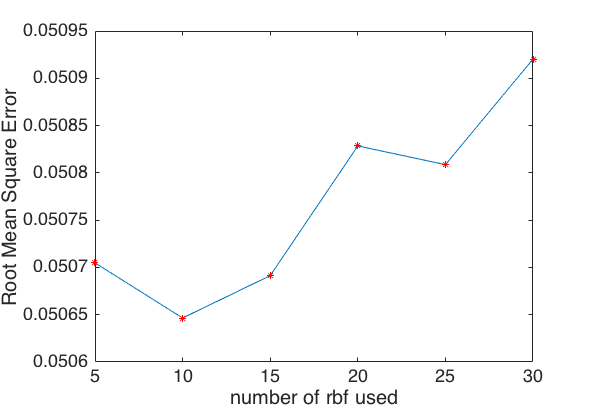
\includegraphics[width=\linewidth]{images/p1-3-a_5_30_another.png}
				 			\caption{}
				 			\label{fig:p-1-3-a_b}
				 		\end{subfigure}\\
				 		\begin{subfigure}{0.5\textwidth}
				 			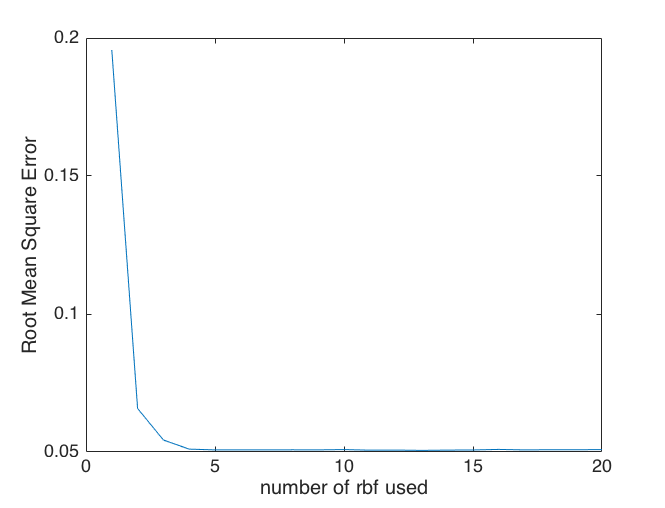
\includegraphics[width=\linewidth]{images/p1-3-a_1_20.png}
				 			\caption{}
				 			\label{fig:p-1-3-a_c}
				 		\end{subfigure}

				 	\end{figure}	
				 	When I ran cross validation procedure to determine which number of radial bases functions among \{ 5, 10, 15, 20, 25, 30\} produces the best results, each time I received a different answer.  The figure \ref{fig:p-1-3-a_a} suggests 5 as the best number of radial bases functions and \ref{fig:p-1-3-a_b} proposes 10 as the best choice. This happens probably due to the random numbers as matlab crossval uses them each time to divide input set on training and validation sets and rbf network initialises weights differently depending on the random numbers. After that I launched the procedure for number of radial basis functions between 1 and 20, and I have realised that it was just a matter of scale. The figure \ref{fig:p-1-3-a_c} demonstrates that we achieve almost no improvement if we use more than 5 radial bases functions in this task. That is why I have chosen 5 as my number of radial basis functions because for the same efficiency it takes less time to compute.
				 	Code snippet for this task:
				 	\lstinputlisting{code/tsk1_3_a.m}
				 \item
					the RMSE for test and training sets:
					\begin{center}
						\begin{tabular}{| c | c | c |}
							\hline
							\, & Training set & Test set \\ \hline
							RMSE  & $0.0506 \pm 0.0010$ & $0.0503 \pm 0.0017$ \\ 
							\hline
						\end{tabular}
					\end{center}
					As it can be seen that radial basis functions don't give any noticeable improvement in comparison to linear regression when both of them are using only adjacent pixels as features.\\ \\ \\ \\
				 	Code snippet for this task:
				 	\lstinputlisting{code/tsk1_3_b.m}
			\end{enumerate}
			 
		\subsection{Linear regression with all pixels}
			the RMSE for test and training sets:
			\begin{center}
				\begin{tabular}{| c | c | c |}
					\hline
					\, & Training set & Test set \\ \hline
					RMSE  &  $0.0371 \pm 0.0007$ & $0.0456 \pm 0.0018$ \\ 
					\hline
				\end{tabular}
			\end{center}
			The RMSE on the training set has dropped significantly comparing to previous models with only adjacent pixels but the improvement one the test set is relatively small. Which may indicate that the complexety of the model has become larger than it is needed for our task. Overall, it is possible to conclude that whereas knowledge of all the pixels helps to predict the value of target pixel better, it seems that the most significant features are pixels adjacent to the target one.
			Code snippet for this task:
			\lstinputlisting{code/tsk1_4.m}
		\subsection{Neural Network with all pixels}
			\begin{enumerate}[label=(\alph*)]
				\item
					the RMSE for test and training sets:
					\begin{center}
						\begin{tabular}{| c | c | c |}
							\hline
							\, & Training set & Test set \\ \hline
							RMSE  & $0.0333 \pm 0.0006$ & $0.0473 \pm 0.0017$ \\ 
							\hline
						\end{tabular}
					\end{center}
					In comparison to linear regression with all pixels Neural Network (NN) slightly over-fits the data because  its error is lower on training set but the error on test set is larger. In my opinion, this happens because NN with all pixels is very sophisticated model for our task.\\
					Code snippet for this task:
					\lstinputlisting{code/tsk1_5_a.m}
					
				\item
					Neural Network RMSE for different random seeds:
					\begin{center}
						\begin{tabular}{| c | c | c |}
							\hline
							Random seed & RMSE on full training set & RMSE on test set\\ \hline
							2015 & $0.0500 \pm 0.0009$ & $0.0515 \pm 0.0014$ \\ 
							2016 & $0.0477 \pm 0.0009$ & $0.0504 \pm 0.0014$ \\ 
							2017 & $0.0485 \pm 0.0009$ & $0.0515 \pm 0.0014$ \\ 
							2018 & $0.0477 \pm 0.0009$ & $0.0516 \pm 0.0014$ \\ 
							2019 & $0.0489 \pm 0.0009$ & $0.0527 \pm 0.0016$ \\
							\hline
						\end{tabular}
					\end{center}
					In comparison to previous task 1.5.a the difference between the errors on the full training set and test set is much smaller in all cases because we are using only 5000 instances from training set for learning and that is why NN is not able to fit all the data points from the full training set. At the same time, most likely due to the same reason, our performance on the full training and test sets has dropped. \\
					Random seed determines to what local minimum NN will try to converge and the starting point from which it will try to converge. So depending on random seeds some runs will be converging faster than others or potentially they will be able to find better/worse local minimum. It explains why our results differ but taking bounds into consideration our performance on the test set is roughly the same for all runs.\\
					Code snippet for this task:
					\lstinputlisting{code/tsk1_5_b.m}
			\end{enumerate}
		\subsection{Discussion}
		 	\begin{figure}[t]
		 		\centering
		 		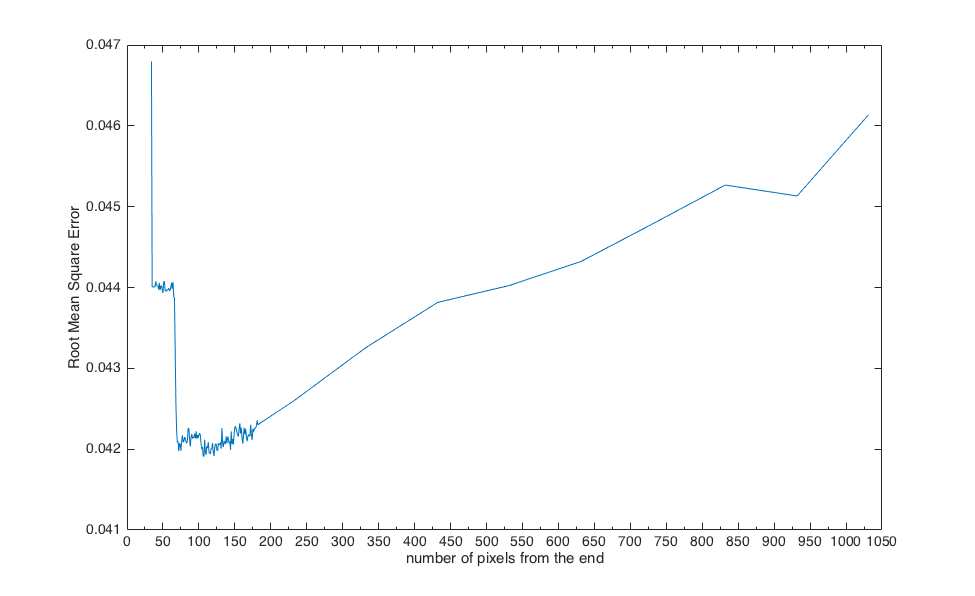
\includegraphics[width=16cm]{images/p1-6_num_pixels.png}
		 		\caption{plot of linear regression RMSE depending on the number of pixels from the end  used as features.}
		 		\label{fig:p1-6_num_pixels}
		 	\end{figure}
		 	\begin{figure}[t]
		 		\centering
		 		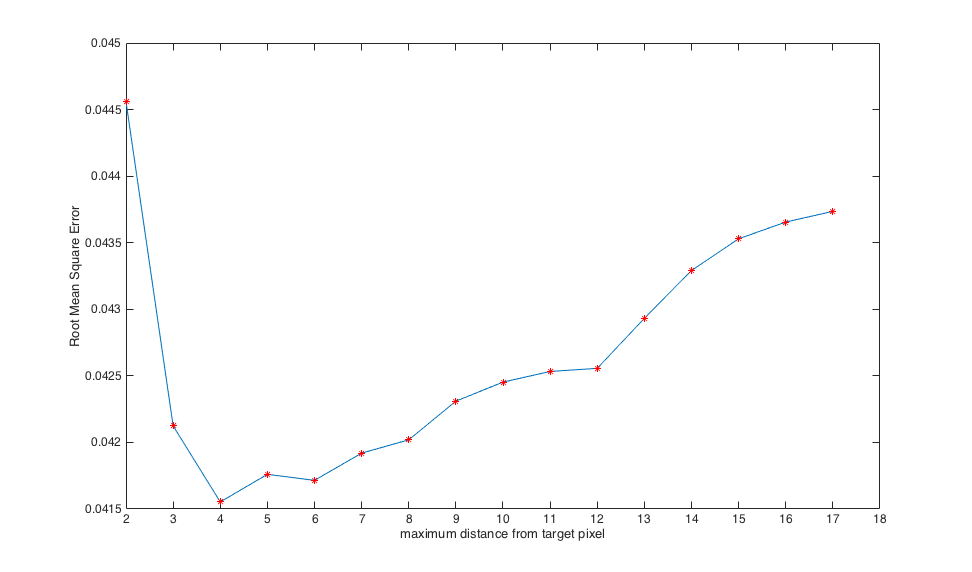
\includegraphics[width=16cm]{images/p1-6_closest_pixels.png}
		 		\caption{plot of linear regression RMSE depending on the maximum distances from the target pixels within which pixels were  used as features.}
		 		\label{fig:p1-6_closest_pixels}	
		 	\end{figure}
		 	In previous tasks linear regression with all pixels showed the best performance. That is why I thought that it would be reasonable to try something else with linear regression. First of all there was noticeable gap between performance of linear regression with all pixels on training set and test set. So we should constraint it somehow.  It seemed to me that the closet pixels to the target one have the biggest impact on the intensity of the target pixel. But how many nearest pixels do we need? I wasn't sure so I evaluated linear regression performance depending on the number of pixels from the end of feature vector via cross-validation on the training set. The result can be seen on the figure \ref{fig:p1-6_num_pixels}. \textbf{Note}: the plot step is not uniform, after 182 I used much bigger step (100) because otherwise cross-validation would take too much time.\\ Figure suggests that the best value from the end is something like 120. Using that number of feature on the test set (xte\_nf(:, 912:1032)) I received the following RMSE:
			\begin{center}
				\begin{tabular}{| c | c | }
					\hline
					\, &  Test set \\ \hline
					RMSE & $0.0419 \pm 0.0017$ \\ 
					\hline
				\end{tabular}
			\end{center}
			
			This result shows improvement in comparison to the previous models. Also we can see that at the beginning figure \ref{fig:p1-6_num_pixels} has form similar to the step function. I describe it by the fact that with period of 35 we receive pixels which are above the target one and they give a lot of information about target pixels. This leads to conclusion that if image is 2d-array of pixels where i, j are indexes on the X and Y axis respectively then we should select pixels/features depending on their euclidean distance from the target pixel $r = \sqrt{(18 - i)^2 + (30 - j)^2}$. \\
			 I have performed cross-validation on the training set to find the best such distance $r$, the results are on figure \ref{fig:p1-6_closest_pixels}. It points out that the best distance is 4, and after checking it on the test set:
			\begin{center}
				\begin{tabular}{| c | c |}
					\hline
					\, &  Test set \\ \hline
					RMSE & $0.0412 \pm 0.0017$ \\ 
					\hline
				\end{tabular}
			\end{center}
			This is good result and this model is computationally efficient because it needs to take only 21 closest pixels in contrast to linear regression or Neural Network with all the pixels. \\ 
			Code snippet to plot figure \ref{fig:p1-6_num_pixels}:
			\lstinputlisting{code/tsk1_6_1.m}
			Code snippet to get performance on the test set using 120 pixels from the end:
			\lstinputlisting{code/tsk1_6_2.m}
			Code snippet to get the closest pixels:
			\lstinputlisting{code/get_closest_pixels.m}
			Code snippet to plot figure \ref{fig:p1-6_closest_pixels}:
			\lstinputlisting{code/tsk1_6_3.m}
			Code snippet to get performance on the test set with pixels within radius 4 from target one:
			\lstinputlisting{code/tsk1_6_4.m}
			\newpage
			
		\section{Robust modelling}
			\section*{Note}
				It is assumed that I have loaded the code from \href{http://www.inf.ed.ac.uk/teaching/courses/mlpr/2015/assignment/part2_code_data.tar.gz}{part2\_code\_data.tar.gz} in my matlab environment. I have also taken professor Iain Murray code from MLPR tutorial 5 to produce error bars - \href{http://homepages.inf.ed.ac.uk/imurray2/code/imurray-matlab/errorbar_str.m}{errobar\_str.m}. text\_data.mat is assumed to be loaded as well.
			\subsection{Fitting the baseline model}
				\begin{enumerate}[label=(\alph*)]
					\item
						\textbf{Bias feature} \\
						The code snippet to add bias term:
						\lstinputlisting{code/tsk2_1_a.m}
					\item
						\textbf{ Maximizing the likelihood} \\
						The code snippet to report logistic regression performance with error bars:
						\lstinputlisting{code/report_lr.m}
						The code snippet for this and next task:
						\lstinputlisting{code/tsk2_1_bc.m}
						I set initial weights to zeros as my starting point in minimisation procedure, because in that case linear regression is unbiased and will give equal probabilities to both labels for any data point. In other words,  it will start as a baseline predictor $P(y | \vect{x}) = 0.5$.\\
						I have received the following results:
						\begin{center}
							\begin{tabular}{| c | c | c |}
								\hline
								\, &  Training set & Test set \\ 
								\hline
								Accuracy                  & $83.35 \pm 0.46 \%$ & $90.71 \pm 0.72 \%$ \\ 
								\hline
								Mean log probability &$-0.4398 \pm 0.0081$ & $-0.299  \pm 0.011  $ \\
								\hline
							\end{tabular}
						\end{center}
						Not a typo, my accuracy was better on the test set. Probably this indicates that training set is noisy (has some mislabelled records) but logistic regression is robust enough to capture general pattern instead of fitting the noise. And if we suggest that the test set was created more carefully then it will explain better accuracy on the test set.
						\\
						The minimisation function converged by itself (I put very big value for maximum number of linear searches - 8000) on 4184 linear search.  The log probability of the baseline line for each input is $log(P(y | \vect{x})) = log(0.5) = -0.6931$. The closer $mean(log(P(y|\vect{x})))$ to zero the more confident predictor in the right answers. Although we must remember the fact that we can have good predictor with good accuracy, but if it gives chances which is close to zero to the right answer even to the one data point then due to the nature of log function ($log(01)= -\infty$) our log mean quantity will be skewed heavily and much smaller than zero. So theoretically it is possible to have predictor with 99.99\% accuracy but with mean log probability far below zero.
						\\
						As we can see our mean log probability in  test set is closer to 0 than those of simple baseline $P(y | \vect{x})=0.5$ which together with our accuracy  implies that our performance is better.
						
					\item
						\textbf{Limited training data}\\
						As in the previous subtask I used zeros as my initial weights (the main code is from previous subtask as well).\\
						For limited number of training examples, my results are:
						\begin{center}
							\begin{tabular}{| c | c | c |}
								\hline
								\, & First 100 points from training set & Test set \\ 
								\hline
								Accuracy                  & $99.0 \pm 1.0 \%$ & $ 75.2 \pm 1.1 \%$ \\ 
								\hline
								Mean log probability &$-0.0139 \pm 0.0098$ & $-\infty$ \\
								\hline
							\end{tabular}
						\end{center}
						From the table it can be see that linear regression fitted the training data too well and it possibly fitted the noise as well.  That is why it has extremely good accuracy and mean log probability close to zero on the training set (it is very confident in its predictions). On other hand, the results on the test set is much worse in comparison to the previous task.  The mean log probability is $-\infty$ which indicates that in some cases our predictor gives zero chances to the right labels from the test set. The accuracy on the test is still better than those of simple baseline $P(y | \vect{x})=0.5$ which means that even from so limited and noisy data for learning, linear regression is able to infer some useful pattern.
						\\
						I had a question how is that possible that accuracy is not 100\% on the limited training set. Dimensionality of our feature vector is 100 (101 with bias), so any binary classification task when we have no more than 100 instances should be perfectly linearly separable. The minimisation function converged on 186 iteration with value 1.386294, but in case of perfectly linearly separable data it must be zero (see  Kevin P. Murphy. Machine Learning  A Probabilistic Perspective. paragraph 8.4.3 - Gaussian approximation for logistic regression). So I decided investigate it further. 
						\\
						The $99.0\%$ accuracy indicates that logistic regression was not able to classify one point correctly from the first 100 instances of the training set. 
						Using the following script I found that due to the some wrong labels in the test data it is possible to have two data points which have the same $\vect{x}$ values but opposite labels:
						\lstinputlisting{code/tsk2_1_c_investigation.m}
						The data points with indices 1 and 21 in the training set are such example. After I threw away the first data point from training set I received the following results:
						\begin{center}
							\begin{tabular}{| c | c | c |}
								\hline
								\, & points from 2 to 100 on training set & Test set \\ 
								\hline
								Accuracy                  & $100 \pm 0.0 \% $ & $ 74.8 \pm 1.1  \%$ \\ 
								\hline
								Mean log probability &$ 0 \pm 0.000$ &  $ -16.0 \pm 1.0 $ \\
								\hline
							\end{tabular}
						\end{center}
						The minimisation function converged on 122 linear search with value 0. This and results in the table lead to conclusion that our training set is perfectly linearly separable. Interesting that our prediction accuracy on the test set dropped slightly, but we have  finite mean log probability on the test at least. But mean log probability is still very small (in comparison to baseline $P(y | \vect{x})=0.5$, for example) which indicates that predictor is too confident and sometimes it makes big mistakes. 
						\\
						Overall this small investigation helped me to understand what kind of noise we have in the training data. 
				\end{enumerate}
			\subsection{Label noise model}
				\begin{enumerate}[label=(\alph*)]
					\item 
						\textbf{Modifying the likelihood}\\
						The events $s_{n}=1$ and $s_{n}=0$ are mutually exclusive and together they are collectively exhaustive events and also  $s_{n}$ is independent from $\vect{x},\ \vect{w},\ y$ that is why:
						\begin{align*}
							P(s_{n}=1) &= 1 - \epsilon \quad P(s_{n}=0)=\epsilon
							\\
							P_{uniform}(y) &= \frac{1}{size(\{-1, +1\})}=\frac{1}{2}
							\\
							P(y|\vect{x},\vect{w}) &= \sigma(y\vect{w}^{T}\vect{x})
							\\
							P(y|\vect{x}, \vect{w}, \epsilon) &= P(s_{n}=1)P(y|\vect{x},\vect{w}) + P(s_{n}=0)P_{uniform}(y)=
							\\
							&=(1-\epsilon)\sigma(y\vect{w}^{T}\vect{x}) + \frac{\epsilon}{2}
						\end{align*}
						
						The derivatives of new model likelihood are:
						\begin{align}
							v^{(n)} &= y^{(n)}\vect{x}^{(n)T}\vect{w}
							\\
							L(\vect{w}, \epsilon) &= \sum_{n=1}^{N}log(P(y^{(n)}|\vect{x^{(n)}}, \vect{w}, \epsilon)) = 
							\sum_{n=1}^{N}log((1-\epsilon)\sigma(v^{(n)}) + \frac{\epsilon}{2}) 
							\\
							\nabla_{\vect{w}}\sigma(v^{(n)}) &= 
							\frac{-1} {(1 + exp(-v^{(n)}))^2} exp(-v^{(n)}) (-1) y^{(n)} \vect{x}^{(n)T} 
							= \sigma^2(v^{(n)}) exp(-v^{(n)}) y^{(n)}\vect{x}^{(n)T}
							\\
							\nabla_{\vect{w}}L(\vect{w}, \epsilon) &= 
							\sum_{n=1}^{N}
								\frac
									{ (1 - \epsilon) \sigma^2(v^{(n)}) exp(-v^{(n)}) y^{(n)} \vect{x}^{(n)T} } 
									{ P(y^{(n)}|\vect{x^{(n)}}, \vect{w}, \epsilon) }				
							\\
							\frac{\partial L(\vect{w}, \epsilon)}{\partial \epsilon} &=
							 \sum_{n=1}^{N} 
								 \frac 
									 {-\sigma(v^{(n)}) + \frac{1}{2}} 
									 {P(y^{(n)}|\vect{x^{(n)}}, \vect{w}, \epsilon)}		
						\end{align}
						I have chosen the following test case for checking gradients implementation:
						\begin{align*}
							\vect{x}^{(1)} = \left(\begin{matrix} 0\\ 0\\ 1 \end{matrix}\right)
							&\quad
							y^{(1)} = -1
							\\
							\vect{x}^{(2)} = \left(\begin{matrix} 2\\ 2\\ 1 \end{matrix}\right)
							&\quad
							y^{(2)}=1 
							\\
							\vect{w} = \left(\begin{matrix} 1\\ 1\\ 1 \end{matrix}\right)
							&\quad
							\epsilon = 0.2
						\end{align*}
						I have used $h =0.1$ which implies that absolute value of error should not exceed 0.01.\\ 
						The results of checking "label noise model" likelihood derivatives via checkgrad.m are:
						\begin{center}
							\begin{tabular}{| c | c | c | c |}
								\hline
								\, & derivative & finite difference & absolute error \\
								\hline
								$w_{1}$ 	& 0.0119 & 0.0120 & 0.0001 \\
								\hline
								$w_{2}$     & 0.0119 & 0.0120 & 0.0001 \\
								\hline
							    $w_{bias}$ &-0.4931 &-0.4928& 0.0003 \\
							    \hline
							    $\epsilon$ & 0.1818 & 0.1825 & 0.0008 \\
							    \hline
							\end{tabular}
						\end{center}
						As we can see in each case the absolute error doesn't exceed 0.01. So our gradient must work fine. As a sanity check I use the fact that test case is symmetric in terms of $w_{1}$ and $w_{2}$, so our derivatives and finite differences for $w_{1}$ and $w_{2}$ must be the same. The absolute error of $\epsilon$ is the biggest one possibly because the step h=0.1 is just too big for it. \\
						Code snippet for "label noise model" log likelihood (will also be used in the next task):
						\lstinputlisting{code/nlm_loglike.m}
						Code snippet for this task:
						\lstinputlisting{code/tsk2_2_a.m}
						
					\item
						\textbf{Fitting a constrained parameter}\\
						Slightly modifying formula (5) from previous task so we can adapt the code from previous example:
						\begin{align*}
						\frac{\partial L(\vect{w}, \epsilon)}{\partial a} &=
						\frac{\partial L(\vect{w}, \epsilon)}{\partial \epsilon} 
						\frac{\partial \epsilon}{\partial a} =
						\sum_{n=1}^{N} 
							\frac 
								{-\sigma(v^{(n)}) + \frac{1}{2}} 
								{P(y^{(n)}|\vect{x^{(n)}}, \vect{w}, \epsilon)}		
							\frac{-1} {(1 + exp(-a))^2} exp(-a) (-1) 
						\\
						&=\sum_{n=1}^{N} 
								\frac 
									{-\sigma(v^{(n)}) + \frac{1}{2}} 
									{P(y^{(n)}|\vect{x^{(n)}}, \vect{w}, \epsilon)}		
							\sigma^2(a)	exp(-a)		=
							\frac{\partial L(\vect{w}, \epsilon)}{\partial \epsilon} 
							\epsilon^2 exp(-a)					
						\end{align*}
						After training label noise model and applying final weights from it on the logistic model, the  performance is:
						\begin{center}
							\begin{tabular}{| c | c | c |}
								\hline
								\, & Training set & Test set \\
								\hline
								Accuracy & $85.17 \pm 0.44\%$ & $91.32 \pm 0.70\%$ \\
								\hline
								Mean Log Probability & $-9.60 \pm 0.47$ & $-1.09 \pm 0.18 $\\
								\hline
							\end{tabular}
						\end{center}
						 From here we can see that accuracy has improved on both training and test sets in comparison to the results from task 2.1.b . Although by looking at the mean log probability for training and test set we can conclude that predictor has become less confident in some cases. But by taking into consideration the fact that our training set contains mislabelled data the predictor should be uncertain about such data points.\\ The better accuracy and thus, classification performance points out that by using model which reflects the condition of  our data set better (mislabelled data) we can infer more useful information from the data set and make our predictor more robust to incorrect data points.
				\end{enumerate}
				
				
\end{document}
